\section{Optimering}
Nu er systemet sat sammen og skal til at optimeres og korrigeres til en ønsket respons. I første omgang er denne ønskede respons så flad så muligt ned til omkring 50Hz. For at se hvad udgangspunktet for højtaleren med enhederne indsat i det modificerede kabinet med basrefleks, og det valgte delfilter laves at frekvenssweep (1 meter afstand) for at se hvordan frekvenskarakteristikken ser ud. Dette kaldes også standard konfigurationen (config 1).  
Udgangspunktet for venstre side af højtaleren kan ses i \autoref*{fig:Standard-udgangspunkt}

\begin{figure}[H] 
	\center
	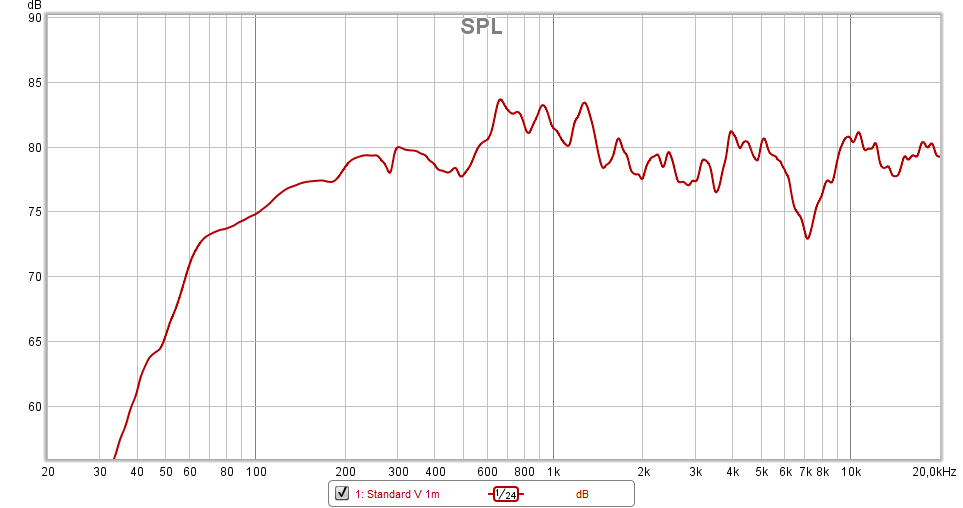
\includegraphics[width=1\linewidth]{figur/Standard-udgangspunkt}\quad
	\caption{Frekvenskarakteristik af venstre side udgangspunkt}
	\label{fig:Standard-udgangspunkt}
\end{figure}

Det kan i \autoref{fig:Standard-udgangspunkt} ses at den akustisk kortslutning forsvundet efter enhederne er kommet i kabinet. For generelt at gøre responsen flad kræver det at frekvenserne for basenheden under 400-500Hz forstærkes/boostes især ved omkring 60Hz, hvis responsen skal være flad ned til omkring 50Hz. Derudover skal frekvenserne for diskanten generelt også hæves en smule, så det udligner det amplitude peak mellem 600hz og 1200 Hz. 


\subsection{Korrektion af enheder}
For at opnå den ønskede frekvensrespons for højtaleren skal bassen korrigeres og diskanten hæves lidt. Derfor laves der i på MiniDSP'en et parametrisk EQ filter (IIR) til at booste/korrigere bassen hos basenhederne og ligeledes et parametrisk EQ filter (IIR) til at løfte diskanterne lidt op i amplitude. Dette kan ses i \autoref{fig:bassboost} og \autoref{fig:diskantboost}. 

\begin{figure}[H]
	\center
	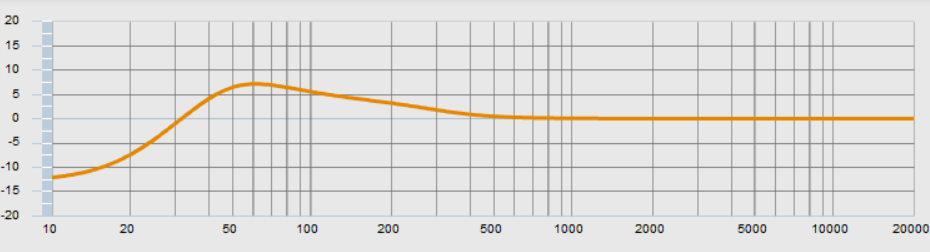
\includegraphics[width=0.9\textwidth]{figur/bassboost}
	\caption{Frekvenskarakterstik for det parametriske EQ filter for basenhederne}
	\label{fig:bassboost}
\end{figure}

\begin{figure}[H]
	\center
	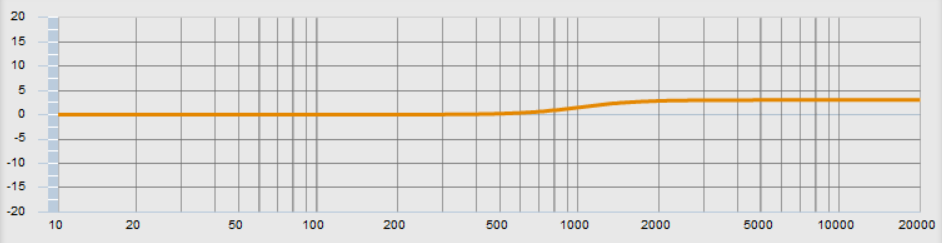
\includegraphics[width=0.9\textwidth]{figur/diskantboost}
	\caption{Frekvenskarakterstik for det parametriske EQ filter for diskantenhederne}
	\label{fig:diskantboost}
\end{figure}

Det parametriske EQ filter for basenhederne i \autoref{fig:bassboost} består af 3 bånd. Første bånd er et low-shelf filter med en Q-værdi på 0.7, som hæver alle frekvenser under 300Hz med 3dB. Andet bånd er også et low-shelf filter med en Q-værdi på 0.7, som dæmper alle frekvenser under 30Hz med 16dB for at beskytte enheden imod for store udsving af membranen ved de helt lave frekvenser. Det sidste bånd består af peak filter med en Q-værdi på 0.7 som hæver frekvenser omkring 60Hz med 6dB. Dette skulle gerne give en nogenlunde flad respons ned til omkring 50-60 Hz og dermed give betydelig mere bas og trommer i lydbilledet. 

Det parametriske EQ filter for diskantenhederne i \autoref{fig:diskantboost} består blot af 1 bånd. Dette bånd er et high-shelf filter med en Q-værdi på 0.7, som hæver alle frekvenser over 1kHz med 3dB. Dette betyder blot at hele diskantens bidrag hæves med 3dB generelt, hvormed de høje toner bliver mere tydelige. Resultatet af denne optimeret konfigurationen (config 2) kan ses i frekvenssweepet (1 meter afstand) på \autoref{fig:Optimering-forskel}, hvor basrefleksen også prøves at lukkes for at se forskellen med og uden basrefleks med det optimeret design. 
\begin{figure}[H] 
	\center
	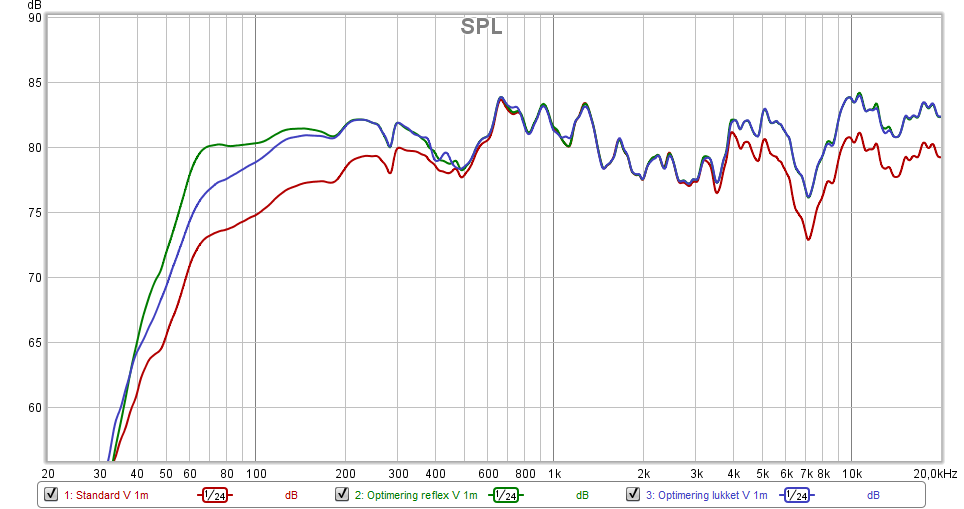
\includegraphics[width=1\linewidth]{figur/Optimering-forskel}\quad
	\caption{Frekvenskarakteristik af venstre side med Optimering/korrektion, Rød = venstre udgangspunkt med åben basrefleks, Grøn = venstre side optimeret med åben basrefleks, Blå = venstre side optimeret med lukket basrefleks}
	\label{fig:Optimering-forskel}
\end{figure}
Som det kan ses i \autoref{fig:Optimering-forskel} er forskellen tydelig med eller uden de to parametriske EQ filter til at korrektion. Hvis man ser på den grønne kurve (optimeret med åben basrefleks) i forhold til den røde kurve (udgangspunkt med åben basrefleks) er frekvensreposen nu flad fra 60Hz-20KHz $\pm3dB$. Derudover er der cirka 6dB forstærkning ved 50Hz og cirka 4dB forstærkning ved 40Hz for den grønne kurve i forhold til den røde kurve, som burde give mere dyb bas. Hvis basrefleksen lukkes mister højtaleren lidt forstærkning omkring 60-70Hz. Derfor må basrefleksens egenresonans ligge heromkring og bidrager altså med 3dB "gratis" forstærkning heromkring. Da vi ikke hverken har designet kabinettet eller basrefleksen til dette system, så er det kun positivt, at den faktisk hjælper med 3dB ekstra lydtryk ved disse frekvenser, som netop bruges flittigt ved et festivalanlæg pga. stortromme og bas præget musik.     

Tilsvarende måling kan laves for højre side, som tilnærmelsesvis ligner venstre side udover nogle små afvigelser ved diskanten . Dette kan ses under bilag i \autoref{fig:Optimering-forskel-VH}. Det samlede resultat for begge højtalere samlet kan også ses under bilag i \autoref{fig:Samlet-Optimering}. I det samlede resultat er det dog værd at bemærke, at en destruktiv interferens opstår omkring 4kHz og 20kHz, da det var svært at placere mikrofonen præcist lige langt mellem de to 2 diskantenheder. Men denne samlede måling er også mere til for at få et indtryk af, hvordan responses ser ud med begge højtalere tilkoblet fx på en festival.

\subsection{EQ af med FIR filtre}
I og med, at man skal have mulighed vælge to konfigurationer til at equalisere lyden til henholdsvis Rock og Jazz, skal der laves to FIR filtre til dette. Disse filtre overføres til MiniDSP'en og danner grundlag for config 3 og config 4.

Filterne laves i Matlab ved hjælp af funktionen $fir2()$. Dette gøres ved at lave et frekvensvektor med 33 bånd. Frekvensvektoren normaliseres, så frekvenserne ligger mellem 0 og 1, hvor 1 er samlingsfrekvensen. For hver af disse punkter(centerfrekvenser) kan frekvensen enten forstærkes eller dæmpes. Derfor laves der en størrelsesvektor(magnitude) kaldet EQ med samme længde af frekvensvektoren. I denne størrelsesvektor sættes den valgte forstærkning som en slags EQ. Til sidste benyttes funktionen $fir2()$ til at få filterkoefficienterne b for det FIR filter, som netop opfylder de valgte forstærkninger ved de tilhørende normaliserede frekvenser. Da det største FIR filter MiniDSP'en kan lave ved brug er 4 kanaler er et 1024 taps FIR filter, vægles der at lave et filter med 1024 tappe. Da MiniDSP'en importere de 1024 koefficienter lidt specielt, laves koefficienterne tilsidst om til en string array, som kan kopires til en tekstfil og derefter overføres til MiniDSP'en. Den fulde Matlab kode til FIR filtrene kan ses under bilag i \autoref{lst:matlab}
  

Designet af EQ vektorene til filterne forklares herunder


\subsubsection{Rock}
Gennem undersøgelse af litteratur \cite[chapter 12]{HomeStudio}, er der blevet valgt nogle forskellige instrumenter, som forstærkes eller dæmpes for at skabe en bestemt effekt. På tabellen nedenunder ses et overblik over de frekvenser som hhv. boostes og dæmpes, og hvilken effekt det  gerne skulle medføre. Disse effekter er valgt af gruppen, ud fra hvilke effekter gruppen synes er essentielt for rock genrer. Problemet med denne måde at equlize på, er at alle instrumenterne bliver påvirket af de forskellige boost/cut. Der vil i diskussionen blive beskrevet yderligere omkring denne problemstilling. 

\begin{center}
\begin{tabular}{| l | l | l | l |}
\hline
 Frekvens i Hz  & Effekt  & Boost/Cut & Instrument  \\\hline
 60-100 & More bottum end & Boost & Kick drum \\ \hline
 200-250 & Fullness & Boost & Guitar\\ \hline
 315-400 & Less Mud & Cut & Guitar \\ \hline
 500-2k & More beefy & Boost & Guitar\\ \hline
 4k-5k & More precence & Boost & Guitar\\ \hline
 8k-10k & More brigthness & Boost & Guitar \& Cymbals\\ \hline
 10k-20k & More crispness & Boost & Cymbals\\ \hline
 
 
\end{tabular}

\end{center}


Ud fra valget af frekvenser, som skal dæmpes eller forstærkes for denne Rock EQ benyttes Matlab, som tidligere nævnt, til at designe et EQ vektor til brug i det FIR filter, som opfylder disse behov. Dette kan ses herunder i  \autoref{lst:ROCK}.   

\begin{lstlisting}[frame=single, caption={FIR EQ vektor Rock kode},label={lst:ROCK},captionpos=b]
%% Rock
EQ = ones(1,length(fn));
EQ(7:9)=boost6; %60-100 
EQ(12:13)=boost6; %200-250 
EQ(14:15)=cut6; %315-400 
EQ(16:22)=boost3; %500-2000
EQ(25:26)=boost6; %4000-5000
EQ(28:29)=boost6; % 8000-10000
EQ(29:end)=boost3; % 10000-end
\end{lstlisting} 
Hernæst generes koefficienterne til Rock FIR filteret ud fra den tidligere nævnte fremgangsmåde(kan også ses under bilag i \autoref{lst:matlab}, hvilket giver følgende frekvensrespons i Matlab, og som kan ses i  \autoref{fig:FIR-Rock1}

\begin{figure}[H]
	\center
	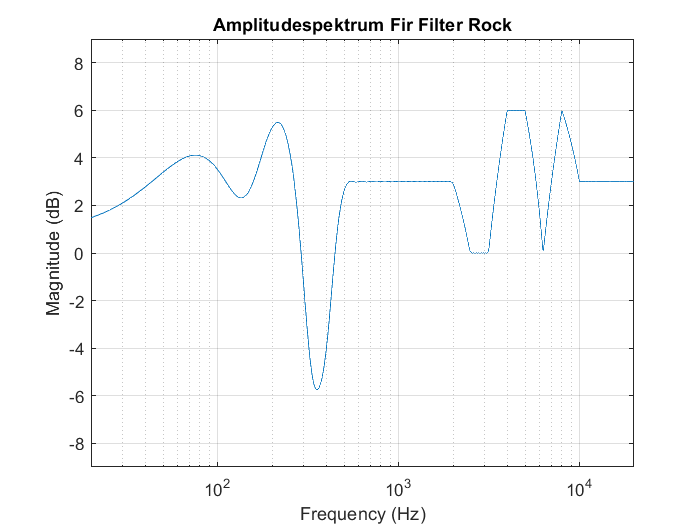
\includegraphics[width=0.9\textwidth]{figur/FIR-Rock1}
	\caption{Frekvenskarakterstik for Rock EQ FIR filteret i Matlab}
	\label{fig:FIR-Rock1}
\end{figure}
I \autoref{fig:FIR-Rock1} ses det at bassen generelt bliver hævet lidt og ligeledes bliver flere bånd af de høje toner hævet lidt. Det ses også, at en del af low-mid båndet dæmpes, hvilket stemmer overens med det tidligere valg af instrumenter og toner, som skulle fremhæves eller dæmpes. Filtret kan også ses overført på MiniDSP'en i \autoref{fig:FIR-Rock2}.

\begin{figure}[H]
	\center
	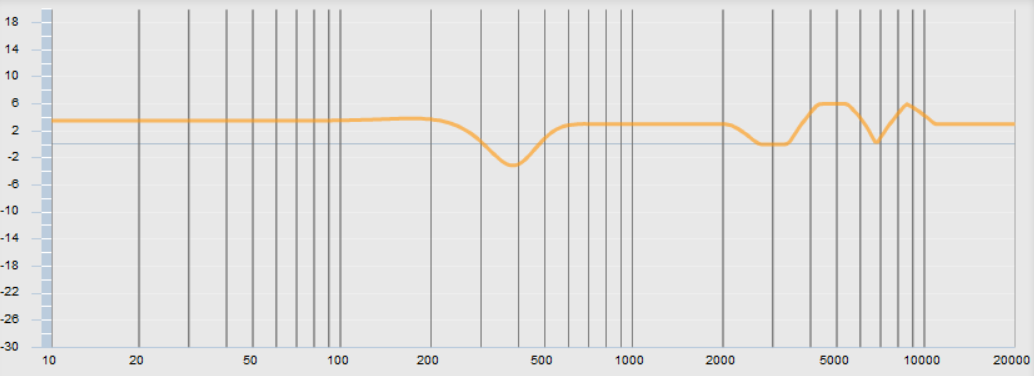
\includegraphics[width=0.9\textwidth]{figur/FIR-Rock2}
	\caption{Frekvenskarakterstik for Rock EQ FIR filteret på MiniDSP'en}
	\label{fig:FIR-Rock2}
\end{figure}
 Her har filteret i \autoref{fig:FIR-Rock2} ændret sig lidt ved frekvenserne under 200Hz i forhold til Matlab versionen. Dette må betyde, at MiniDSP'en ikke har kunne realisere filtret præcist som forventet ved de lave frekvenser og har måske afrundet nogle koefficienter. Generelt set stiger det overordnede lydtryk også med cirka 3dB samlet set. Dette gør, at hele input signalet på MiniDSP'en skal sænkes 3dB, hvis man skal kunne sammenligne denne konfiguration (config 3) med den normale optimerede konfiguration (config 2) rent lydtryksmæssig. Derfor dæmpes indputtes på config 3 med 3dB, så config 3 har omtrent samme lydtryk under lyttetesten som config 2.  

\subsubsection{Jazz}
Gennem undersøgelse af litteratur \cite[chapter 12]{HomeStudio}, er der blevet valgt nogle forskellige instrumenter, som forstærkes eller dæmpes for at skabe en bestemt effekt. På tabellen nedenunder ses et overblik over de frekvenser som hhv. boostes og dæmpes, og hvilken effekt det gerne skulle medføre. Disse effekter er valgt af gruppen, ud fra hvilke effekter gruppen synes er essentielt for jazz genrer. Problemet med denne måde at equlize på, er at alle instrumenterne bliver påvirket af de forskellige boost/cut. Der vil i diskussionen blive beskrevet yderligere omkring denne problemstilling. 

\begin{center}
\begin{tabular}{| l | l | l | l |}
\hline
 Frekvens i Hz  & Effekt  & Boost/Cut & Instrument  \\\hline
 50-100 & low end roll off & Cut & Cymbals \\ \hline
 160-400 & Fullness & Boost & Saxophone\\ \hline
 630-800 & Brightness & Boost & Saxophone \\ \hline
 2k-5k & Presence & Boost & Piano\\ \hline
 8k-10k & Brightness & Boost & Cymbals\\ \hline
 
 
\end{tabular}

\end{center}



Ud fra valget af frekvenser, som skal dæmpes eller forstærkes til for denne Jazz EQ benyttes Matlab, som tidligere nævnt, til at designe et EQ vektor til brug i det FIR filter, som opfylder disse behov. Dette kan ses herunder i  \autoref{lst:Jazz}.   

\begin{lstlisting}[frame=single, caption={FIR EQ vektor Jazz kode},label={lst:Jazz},captionpos=b]
%% Jazz
EQ = ones(1,length(fn));
EQ(6:9)=cut3; %50-100 
EQ(11:15)=boost6; %160-400
EQ(17:18)=boost6; %630-800
EQ(22:26)=boost3; % 2000-5000
EQ(28:29)=boost3; % 8000-10000
\end{lstlisting} 
Hernæst generes koefficienterne til Jazz FIR filteret ud fra den tidligere nævnte fremgangsmåde(kan også ses under bilag i \autoref{lst:matlab}, hvilket giver følgende frekvensrespons i Matlab, og som kan ses i  \autoref{fig:FIR-Jazz1}

\begin{figure}[H]
	\center
	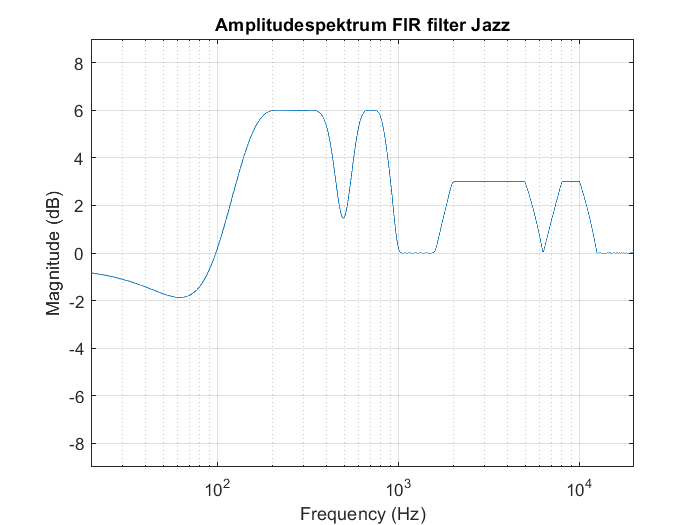
\includegraphics[width=0.9\textwidth]{figur/FIR-Jazz1}
	\caption{Frekvenskarakterstik for Jazz EQ FIR filteret i Matlab}
	\label{fig:FIR-Jazz1}
\end{figure}
I \autoref{fig:FIR-Jazz1} ses det at bassen generelt bliver dæmpet og ligeledes bliver flere bånd i low-mid området fremhævet og nogle af de høje toner bliver også hævet en smule. Derfor stemmer filtret nogenlunde overens med det tidligere valg af instrumenter og toner, som skulle fremhæves eller fjernes. Filtret kan også ses overført på MiniDSP'en i \autoref{fig:FIR-Jazz2}.

\begin{figure}[H]
	\center
	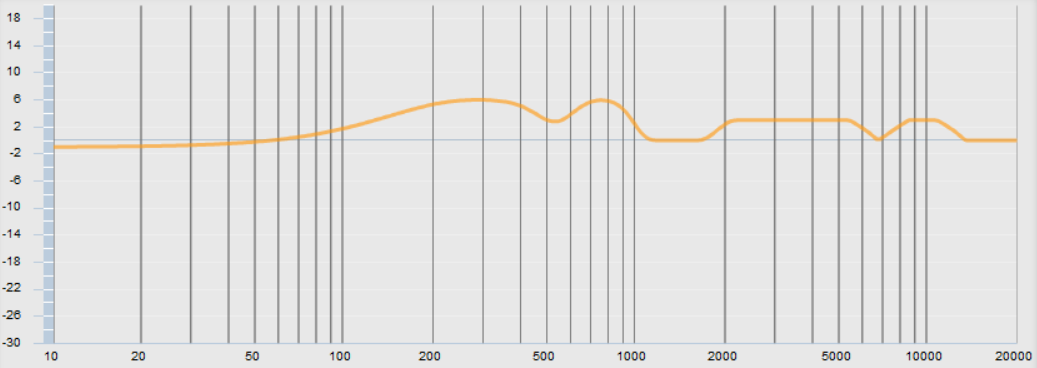
\includegraphics[width=0.9\textwidth]{figur/FIR-Jazz2}
	\caption{Frekvenskarakterstik for Jazz EQ FIR filteret på MiniDSP'en}
	\label{fig:FIR-Jazz2}
\end{figure}
Filteret i \autoref{fig:FIR-Jazz2} stemmer meget overens med Matlab versionen. Der er kun få ændringer i skarpheden af filtret omkring 50-60Hz, som MiniDSP'en ikke har kunne realisere præcist som forventet  Generelt set stiger det overordnede lydtryk også igen med cirka 2-3dB samlet set. Dette gør, at hele input signalet på MiniDSP'en skal sænkes cirka 3dB, hvis man skal kunne sammenligne denne konfiguration (config 4) med den normale optimerede konfiguration (config 2) rent lydtryksmæssig. Derfor dæmpes indputtes på config 4 med også med 3dB, så config 4 har omtrent samme lydtryk under lyttetesten som config 2.  

\subsubsection{Resultat}
For at sammenligne config 2 (Optimeret ), config 3 (Rock) og config 4(Jazz) måles frekvensresponsen for stereo setuppet i det lyddøde rum i 1 meters afstand. Det er ikke den helt optimale målemetode, da det er svært at placere mikrofonen præcist lige langt mellem de nu 2 diskantenheder(og lige langt mellem basenhederne), hvormed der i denne måling opstår en destruktiv interferens omkring 7-8kHz svarende til 2-3cm i afstandsforskel til mikrofonen. Dette betyder dog ikke noget for selve sammenligningen mellem de 3 konfigurationer, da denne interferens skabes ved alle 3 målinger. Derfor viser forskellen mellem de tre målinger blot forskellen mellem de 3 konfigurationer, som vi netop er interesseret i at sammenligne. Resultatet kan ses i \autoref{fig:EQ-forskelle} herunder.


\begin{figure}[H]
	\center
	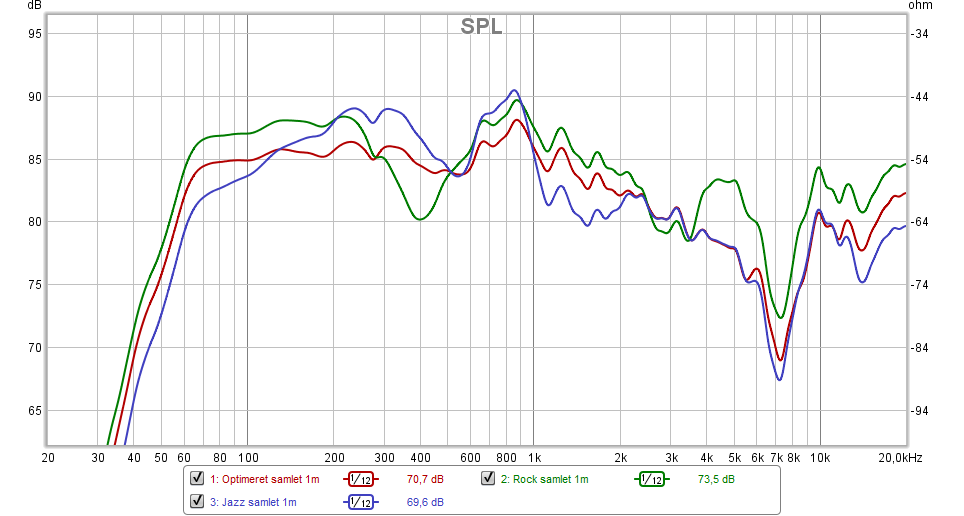
\includegraphics[width=1\textwidth]{figur/EQ-forskelle}
	\caption{Frekvenskarakterstik for stereo opsætning for henholdsvis (Rød) config 2, (Grøn) config 3 og (Blå) config 4}
	\label{fig:EQ-forskelle}
\end{figure}

Som det kan ses i \autoref{fig:EQ-forskelle} så opfører de 3 konfigurationer sig som forventet. Den grønne kurve for Rock giver mere kraft i  bas-båndet mellem 40Hz og 300 Hz, dæmper low-mid båndet omkring 400Hz og hæver flere høje toner for at fremhæve de ønskede instrumenter. Den blå kurve for Jazz dæmper bassen under 100 Hz, forstærker både lidt i det høje bas bånd fra 160-300Hz og i low-mid båndet fra 600-800Hz. Den blå kurve for Jazz dæmper faktisk også de aller højeste toner, hvilket ikke skyldes selve EQ filteret, men derimod den overordnende niveaujustering på -3dB på inputsignalet. 

Så generelt ser resultatet i frekvensresponsen ud som forventet og ønsket, men det virkelige interessante bliver, hvordan resultatet af lyttetesten ser ud for selve oplevelsen af de 3 konfigurationer.     



